\documentclass{article}

% if you need to pass options to natbib, use, e.g.:
\PassOptionsToPackage{numbers, compress}{natbib}
% before loading neurips_2020

% ready for submission
% \usepackage{neurips_2020}

% to compile a preprint version, e.g., for submission to arXiv, add add the
% [preprint] option:
%     \usepackage[preprint]{neurips_2020}

% to compile a camera-ready version, add the [final] option, e.g.:
\usepackage[final]{neurips_2020}

% to avoid loading the natbib package, add option nonatbib:
%\usepackage[nonatbib]{neurips_2020}

\usepackage[utf8]{inputenc} % allow utf-8 input
\usepackage[T1]{fontenc}    % use 8-bit T1 fonts
\usepackage{hyperref}       % hyperlinks
\usepackage{url}            % simple URL typesetting
\usepackage{booktabs}       % professional-quality tables
\usepackage{amsfonts}       % blackboard math symbols
\usepackage{nicefrac}       % compact symbols for 1/2, etc.
\usepackage{microtype}      % microtypography
\usepackage{array,multirow,graphicx}
\usepackage{amsmath}
\usepackage{arydshln}

\usepackage{adjustbox}

\usepackage{pgfplots}
\usepackage{filecontents}
\usepackage{pgfplotstable}

\title{Rectified Convolution}

% The \author macro works with any number of authors. There are two commands
% used to separate the names and addresses of multiple authors: \And and \AND.
%
% Using \And between authors leaves it to LaTeX to determine where to break the
% lines. Using \AND forces a line break at that point. So, if LaTeX puts 3 of 4
% authors names on the first line, and the last on the second line, try using
% \AND instead of \And before the third author name.

\author{%
  Hang Zhang \\
  Amazon \\
  \texttt{hzaws@amazon.com} \\
}

\begin{document}

\maketitle

\begin{abstract}
  
  We propose a simple modification of the convolutional layer by rectifying the feature-map activations, which alleviates the biases introduced via zero-padding. We refer to this modified version of convolution as {\em rectified convolution}. 
  Comparing to standard convolutional layer, the rectified version almost introduces no extra computation cost or memory usage. 
  Simply replacing the convolutional layer with the rectified version, the performances of CNNs are consistently improved, for example the top-1 accuracy of ResNet-50 on ImageNet is increased from 76.5\% to 77.1\%. %\footnote{Despite the improvement is small, this non-biased representation could be potentially helpful for the other applications (such as alleviating artifacts of output images from generative model, and improving boundaries of semantic segmentation).}
  
  
\end{abstract}

\section{Introduction}

% CNN
% large trianing crop size necessary?

Convolutional neural network (CNN) has become the pre-dominant method in computer vision. 
CNN learns the feature representation directly from the data by stacking the convolutional layers with non-linearities and downsampling. 
There are a lot of research study on non-linearity functions and regularization methods, but the convolutional layer has stayed almost unchanged since LeNet~\cite{lecun1998gradient}. In this paper, we rethinking the boundary padding for convolutional layers. % and alleviates the biases introduced by zero padding.


% . what is the correct padding value? boundary misalignment.
Modern CNN architectures often follow a modular design which stacks multiple blocks in the same type at each stage~\cite{simonyan2014very,he2015deep}. 
To preserve the same spatial resolution at each stage, zero-padding is used for convolutional layers. 
However, the input feature-map is often ReLU activated with a non-zero mean. 
As convolutional layers act in a sliding window manner, the resulting activations along the feature-map boundaries have padded zeros as the input, which makes it hard to estimate the batch statistics reliably using Batch Normalization. 
In addition, the ratio between the boundary pixels and the interior pixels change with the input size, which may lead to discrepancy in the feature representation using different training and validation image resolutions~\cite{touvron2019fixing}. 


For the image-to-image problem, the generative model often employs reflection-padding to alleviates the artifacts along the boundaries due to the padding~\cite{zhang2017multistyle}. 
Despite its success in generative model, the reflection-padding is not suitable for image classification network due to introducing aliasing artifacts. 
A question naturally arises {\it what is the idea padding value along the feature-map boundaries}? Dropout~\cite{srivastava2014dropout} randomly masks out ratio $p$ of the activations in the feature-map, and scales up the remaining activations by $\frac{1}{1-p}$ during the training. 
And it serves as an identity layer during the inference to form a in-network ensemble of various modes during the training. Inspired by the dropout work, we treat the padded zeros as the missing pixels just like being masked out along the boundaries. 


% Dropout. In-network ensemble. 
% DropBlock
% Boundary dropout

\begin{figure}[t]
    \centering
    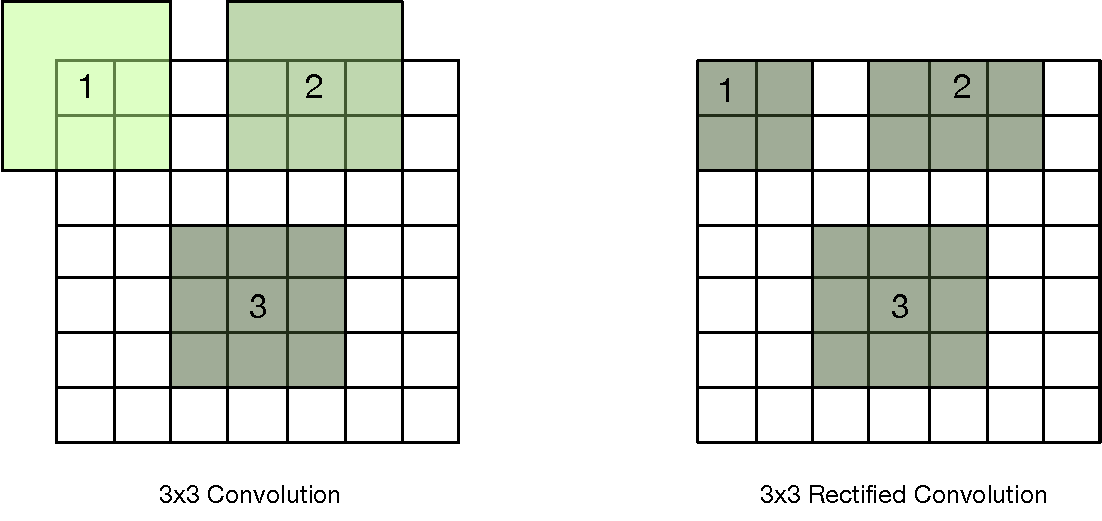
\includegraphics[width=0.9\linewidth]{fig/rectified_conv.pdf}
    \caption{Comparing to the standard 2D convolution with zero-padding, rectified convolution only takes the valid input values and scale up the activations based on number of valid input elements. The kernel size is $3\times 3$ and feature-map size is $7\times 7$. 
    %(Using different color to visualize the different number of valid pixels.)
    }
    \label{fig:rectified_conv}
\end{figure}


As the main contribution of this paper, we introduce a {\it rectified convolution}, where the boundary values are rectified to alleviates the biases introduced by zero-padding. 
We simply scale up the activation by a ratio of $\frac{kernel\_size}{valid\_pixels}$ to compensate the padded zeros, so that the expectation of the resulting feature-map mean is consistent across spatial locations. 
Experimental results have shown that the proposed rectified convolution can improve the classification accuracy on ImageNet~\cite{imagenet} consistently for different CNN architectures. 
We have also studied the behavior of using average aggregation mode instead of summation in the convolutional layers, and have achieved similar performance. 
It demonstrates that the discrepancies are mainly caused by unbalanced valid pixel ratio instead of aggregation mechanism. 
This modification is simple and can be easily implemented as an in-place operator using deep learning toolkit~\footnote{PyTorch implementation will be released upon publication.}, with almost no extra computation cost or memory usage.


\section{Methods}


%Convolution is a translation equivariant operation. 

In this section, we use 2D convolution as an example to describe how rectified convolution works. The convolutional layer can be regarded as a 2D convolution if it has stride of 1 and a single input and output channel.

\subsection{2D Convolution with Zero-padding}

For a zero-padded 2D convolution with an input feature-map $x\in\mathbb{R}^{H\times W}$ and kernel $k\in\mathbb{R}^{m\times n}$, the value of the output feature-map $y\in\mathbb{R}^{H\times W}$ at the location $[h, w]$ can be represented as: 

\begin{equation}
    %\begin{aligned}
    y[h, w]=\sum_{i=1}^m\sum_{j=1}^n k[i, j] \cdot \hat{x}[h-i, w-j] ,
    %\end{aligned}
\end{equation}

where $\hat{x}[h, w]$ is the input pixel value at the location $[h, w]$ or padded zero:

\begin{equation}
    \hat{x}[h, w]=
    \begin{cases}
        x[h, w] & \text{if } \delta(x[h, w])\\
        0, & \text{otherwise} ,
    \end{cases}
\end{equation}

where $\delta()$ is an indicator function which indicates whether the pixel is valid (inside the input feature-map):

\begin{equation}
    \delta(x[h, w]) = (0\le h \le H) \land (0 \le w \le W). 
\end{equation}


\paragraph{Boundary Effects and Feature Discrepancy.}

The convolution operation acts in a sliding window manner. The number of valid input pixels inside the convolutional kernel depends on the pixel location of the input, as shown in Figure~\ref{fig:rectified_conv}. 
The input feature-map of convolutional layer in modern CNN is usually ReLU activated and has a non-zero mean. 
The activations along the feature-map boundaries are biased due to zero padding. 
In addition, the ratio of non-biased activations varies with different input sizes. For example 36 pixels are non-biased for input feature-map size of $7\times7$ using a $3\times3$ convolution kernel and resulting in a valid ratio of $36/49=0.735$, while the valid ratio for $6\times6$ is $0.694$. 

Batch normalization~\cite{ioffe2015batch} is often used as a regularization after the convolutional layer in CNNs. The accumulation of batch statistics becomes difficult to establish due to the biased activations along the boundaries. Furthermore, the estimated batch statistics is conditional on the input resolution change, leading to the discrepancy in the learned network representation. 

\subsection{Rectified Convolution}

To tackle the difficulty of inconsistent number of valid input pixels along the feature-map boundaries, we simply scale up the resulting activation: 

\begin{equation}
    y[h, w]=\frac{mn}{v[h, w]}\sum_{i=1}^m\sum_{j=1}^n k[i, j] \cdot \hat{x}[h-i, w-j] ,
\label{eq:rfconv}
\end{equation}

where $v[h, w]$ is the number of valid pixels residing inside the feature-map for the pixel location at $h, w$:

\begin{equation}
    v[h, w]=\sum_{i=1}^m\sum_{j=1}^n\mathbf{1}[(0\le h-i\le H) \land (0 \le w-j \le W)].
\end{equation}


%\paragraph{Feature-map Mean. }




\section{Experimental Results}

In this section, we first compare the image classification performance if different CNN architectures~\cite{he2015deep,xie2016aggregated,zhang2020resnest,radosavovic2020designing} using rectified convolution and standard 2D convolution with zero-padding on ImageNet dataset~\cite{imagenet}, then study the different aggregation mode in the rectified convolution. 

\begin{table}
    \begin{center}
        \begin{tabular} {l | c | l  }
            \toprule[1pt]
            %{\bf Method} 
            {\bf Network} & {\bf Rectified} & {\bf acc\%} \\ 
            \hline
            \multirow{2}{*}{ResNet-50~\cite{he2015deep}} &  & 76.48 \\
            %\cdashline{2-3}
             & \checkmark & 77.10 (+0.62) \\
            \hdashline
            \multirow{2}{*}{ResNet-101~\cite{he2015deep}} & & 78.13 \\
            & \checkmark & 78.74 (+0.41) \\
            \hdashline
            \multirow{2}{*}{ResNeXt-50~\cite{xie2016aggregated}} & & 78.17 \\
            & \checkmark & 78.48 (+0.31) \\
            \hdashline
            % \multirow{2}{*}{ResNeSt-50~\cite{zhang2020resnest}} & & 78.55 \\
            % & \checkmark & 79.17 (+0.62) \\
            % \hdashline
            \multirow{2}{*}{RegNetX-4GF~\cite{radosavovic2020designing}} & & 79.03 \\
            & \checkmark & 79.35 (+0.33) \\
            \hdashline
            \multirow{2}{*}{ResNeSt-50$\dagger$~\cite{zhang2020resnest}} & & 78.73 \\
            & \checkmark & 79.38 (+0.65) \\
            \bottomrule[1pt]
        \end{tabular}
    \end{center}   
\caption{Image classification results on ImageNet. Rectified convolution consistently improves the performance for different CNN architectures. (ResNeSt-50$\dagger$ is using $2s8x$ fast setting with 4.5GFLOPs and 26.4M params.)}
\label{tab:rfconv}
\end{table}



\paragraph{Implementation Detail}

For easily measure the improvement of rectified convolution, we train different network architectures in the same setting. 
We use data parallel training on 8 GPUs with data sharding, where the mini-batch on each GPU is sampled from the corresponding shard without replacement. 
For data augmentation, only standard transformations are used, including random size cropping between 0.08 to 1.0 of the original image area, random horizontal flip, color jittering and lighting changes. 
After jittering, the image is subtracted by RGB mean and divided by the standard deviation before fed into the network. 
Batch Normalization~\cite{ioffe2015batch} and ReLU activation function ~\cite{nair2010rectified} are used after each convolutional layer. 
A mini-batch size of 512 is used with 64 image samples per GPU. 
We use a learning rate of 0.2 and a weight decay of 0.0001. 
No regularization method is used except for weight decay. The networks are trained on the ImageNet training set for 120 epochs with a cosine learning rate decay and evaluated on the validation set. 

\paragraph{Rectified Convolution}

We evaluate the performance of difference CNN models using rectified convolution or standard convolution with zero-padding, including ResNet~\cite{he2015deep}, ResNeXt~\cite{xie2016aggregated}, ResNeSt~\cite{zhang2020resnest} and RegNet~\cite{radosavovic2020designing}.
The image classification top-1 accuracy on ImageNet~\cite{imagenet} validation set is reported in Table~\ref{tab:rfconv}. 
We can see that the performances of these networks are boosted by $0.3-0.6\%$ on top-1 accuracy. 


\paragraph{Sum mode v.s. Average Mode}
Since rectified convolution mainly balances the activation scale regardless of the number of valid input elements, it is naturally to consider using average mode to aggregate the convolution instead of summation. 
In this way, it is the same as averaging the responses only on the valid input elements:

\begin{equation}
    y[h, w]=\frac{1}{v[h, w]}\sum_{i=1}^m\sum_{j=1}^n k[i, j] \cdot \hat{x}[h-i, w-j] ,
\label{eq:rfconv2}
\end{equation}

\begin{table}
    \begin{center}
        \begin{tabular} {l | c | l  }
            \toprule[1pt]
            %{\bf Method} 
            {\bf Network} & {\bf Rectified} & {\bf acc\%} \\ 
            \hline
            \multirow{2}{*}{ResNet-50~\cite{he2015deep}} & sum & 77.10  \\
            %\cdashline{2-3}
             & avg & 77.11 \\
            \bottomrule[1pt]
        \end{tabular}
    \end{center}   
\caption{Sum aggregation v.s. average aggregation. Image classification results on ImageNet. }
\label{tab:sumavg}
\end{table}



$v[h,w]$ is the count of valid input at output location $h, w$ as in Equation~\ref{eq:rfconv}. We compare the performance of ResNet-50 on ImageNet, and the results are shown in Table~\ref{tab:sumavg}. We get very similar performance using different aggregation mode, which demonstrates that the biases are main introduced by inconsistent valid input elements between boundary and interior pixels instead of aggregation mode. 


%\begin{filecontents*}{resnet50.txt}
3.3525657653808594,
 18.373233795166016,
 29.461240768432617,
 35.04364776611328,
 38.38871765136719,
 40.77903747558594,
 42.62984848022461,
 43.79066467285156,
 44.79474639892578,
 45.30116271972656,
 46.11604309082031,
 46.5025634765625,
 46.89033508300781,
 47.45357131958008,
 47.767662048339844,
 48.00681686401367,
 48.20288848876953,
 48.509483337402344,
 48.57692337036133,
 49.10706329345703,
 49.3287353515625,
 49.481719970703125,
 49.470481872558594,
 49.504825592041016,
 50.01810836791992,
 50.10927200317383,
 50.189823150634766,
 50.22167205810547,
 50.63317108154297,
 50.565731048583984,
 50.76804733276367,
 50.993465423583984,
 51.09462356567383,
 51.20077896118164,
 51.55358123779297,
 51.50362777709961,
 51.97319793701172,
 51.8782844543457,
 52.22734069824219,
 52.348480224609375,
 52.22983932495117,
 52.636966705322266,
 52.824920654296875,
 53.16398620605469,
 53.187713623046875,
 53.38191223144531,
 53.34694290161133,
 53.677268981933594,
 53.98573684692383,
 54.14621353149414,
 54.302947998046875,
 54.45780563354492,
 54.56146240234375,
 54.82746887207031,
 55.274559020996094,
 55.35261535644531,
 55.709163665771484,
 55.75474548339844,
 55.95144271850586,
 56.55152130126953,
 56.245548248291016,
 56.697635650634766,
 56.89433288574219,
 57.45756912231445,
 57.37202072143555,
 57.75230026245117,
 57.92464065551758,
 58.3492546081543,
 58.48288345336914,
 58.78385925292969,
 58.96369171142578,
 59.55690383911133,
 59.55003356933594,
 60.05582046508789,
 60.3037223815918,
 60.468570709228516,
 60.996212005615234,
 61.397098541259766,
 61.8566780090332,
 61.82170867919922,
 62.23695755004883,
 62.93257141113281,
 63.10304260253906,
 63.61070251464844,
 63.753074645996094,
 64.09276580810547,
 64.46492004394531,
 64.9875717163086,
 65.49773406982422,
 65.9223403930664,
 66.19334411621094,
 66.75658416748047,
 67.19367980957031,
 67.68698120117188,
 67.91427612304688,
 68.54244995117188,
 69.30675506591797,
 69.62458801269531,
 70.23153686523438,
 70.6973648071289,
 71.05328369140625,
 71.66647338867188,
 72.18787384033203,
 72.65432739257812,
 73.2269287109375,
 73.61470031738281,
 74.31156158447266,
 74.96221923828125,
 75.4673843383789,
 75.85140991210938,
 76.53328704833984,
 76.77182006835938,
 77.190185546875,
 77.5429916381836,
 77.68785858154297,
 77.97384643554688,
 78.0887451171875,
 78.1799087524414,
 78.24422454833984,
 78.3422622680664
 
 
 6.269903659820557,
 23.49605941772461,
 33.35019302368164,
 38.080875396728516,
 40.679752349853516,
 42.79032897949219,
 43.91117858886719,
 44.98082733154297,
 46.03799057006836,
 46.446990966796875,
 46.79792022705078,
 47.39112854003906,
 47.65776062011719,
 48.20726013183594,
 48.40769958496094,
 48.61875915527344,
 48.73615264892578,
 48.96531677246094,
 49.314998626708984,
 49.396175384521484,
 49.93006134033203,
 50.1792106628418,
 50.03683853149414,
 50.12113952636719,
 50.334068298339844,
 50.678131103515625,
 50.78740310668945,
 50.83049011230469,
 51.131465911865234,
 51.265716552734375,
 51.33627700805664,
 51.75777053833008,
 51.78461837768555,
 51.82770538330078,
 52.16302490234375,
 52.12930679321289,
 52.5501708984375,
 52.627601623535156,
 52.52519226074219,
 52.908592224121094,
 53.13713455200195,
 53.152748107910156,
 53.38191223144531,
 53.3238410949707,
 53.76655960083008,
 53.92891311645508,
 54.03444290161133,
 54.09001541137695,
 54.34228515625,
 54.4446907043457,
 54.733177185058594,
 54.87367630004883,
 55.21149444580078,
 55.30141067504883,
 55.64484786987305,
 55.63360595703125,
 55.97079849243164,
 56.279266357421875,
 56.194969177246094,
 56.760704040527344,
 57.03607940673828,
 57.1147575378418,
 57.35765838623047,
 57.707340240478516,
 58.141944885253906,
 58.01643371582031,
 58.30741882324219,
 58.72890853881836,
 59.14789962768555,
 59.40578842163086,
 59.491336822509766,
 59.859127044677734,
 59.91220474243164,
 60.578468322753906,
 60.468570709228516,
 61.150447845458984,
 61.176048278808594,
 61.62314224243164,
 62.135799407958984,
 62.49484634399414,
 62.68404769897461,
 63.12801742553711,
 63.478946685791016,
 63.81863784790039,
 63.98099136352539,
 64.4299545288086,
 64.87642669677734,
 65.43029022216797,
 65.71815490722656,
 66.09343719482422,
 66.37942504882812,
 67.1674575805664,
 67.49465942382812,
 67.93488311767578,
 68.24959564208984,
 68.94271087646484,
 69.47410583496094,
 69.67829132080078,
 70.24340057373047,
 70.85784149169922,
 71.3417739868164,
 71.98431396484375,
 72.52007293701172,
 73.05396270751953,
 73.42050170898438,
 74.08114624023438,
 74.76490020751953,
 75.24446105957031,
 75.73526763916016,
 76.40715026855469,
 76.85736846923828,
 77.20767211914062,
 77.40998840332031,
 77.87518310546875,
 78.08312225341797,
 78.2935562133789,
 78.48150634765625,
 78.50711059570312,
 78.52397155761719,
 78.48150634765625
\end{filecontents*}

\begin{figure}
\centering
\begin{adjustbox}{max height=3.7cm}           
\begin{tikzpicture}
\begin{axis}[
    %xmin=0, xmax=600,
	%ymin=50.0, ymax=82,
	xlabel={epochs},
    ylabel={training accuracy},
    legend style={cells={align=left},font=\small},
    extra tick style={grid style={black},xticklabel=\empty},
    grid=both,
]
\addplot gnuplot [raw gnuplot, mark=none] {plot 'resnet50.txt' index 0};
\addplot gnuplot [raw gnuplot, mark=none] {plot 'resnet50.txt' index 1};
\addlegendentry{standard convolution};
\addlegendentry{rectified convoluton};
\end{axis}
\end{tikzpicture}
\end{adjustbox}
\vspace{-0.8em}
\caption{Train and validation curves of EncNet-32k64d and the baseline Se-ResNet-64d on CIFAR-10 dataset, plotting error rate as a function of epochs. }
\vspace{-0.8em}
\end{figure}

\section{Conclusion}
In this paper, we propose a simple modification of standard convolutional layer with zero-padding by rectifying the activations with padded zero input along the boundaries. We refer to this modified version as rectified convolution. 
The modification is simple yet efficient, and consistently improves the performance of CNNs without introducing extra computation or memory usage. 
As the rectified convolution alleviates the aliasing along the feature-map boundaries, we expect it could be beneficial to generative models or segmentation CNNs. 

\bibliographystyle{splncs04}
\bibliography{egbib}

\end{document}